\documentclass{article}
\usepackage{hyperref}
\usepackage{amssymb}
\usepackage{amsmath}
\usepackage{color,graphicx} 

\begin{document}
\title{Libsvm using GPU}
\author{Anirudhan J. Rajagopalan \\ N18824115 \\ ajr619}
\maketitle

% write about lib svm format (svm light)
% two possible places for optimizations.  
% Calculating the gram matrix
% Porting the Sequential Minimal Optimization to GPU.

% Structures in libsvm
% svm_problem
% svm_node

% lru cache for all the rows processed in the kernel
% svm.cpp dot function (line no. 294). Modifying the dot function is difficult 
% as the internal datastructures has to be changed.

\newpage

\section{Abstract}
This project is an attempt to implement the Support Vector Machine~\cite{cortes1995} classifier using GPUs.
We tried two approaches: 
The first one is to try to port the Sequential Minimal Optimization part to the GPU\@.
The second one is to implement the Gram matrix~\cite{wiki:gram_matrix} calculation to GPUs.
We end up using the second approach and we show show performance improvements over the conventional approach used by libsvm. 
\section{Introduction}
The most popular implementation of SVM is libsvm~\cite{CC01a}.  
It is used in almost all the traditional machine learning applications.
Since it projects data into a higher dimensional space, we were able to solve problems that are not easily classifiable in the lower dimensional space.

Porting a SVM to GPUs will help us use this classifier easily in deep learning models too.
Though deep learning already uses various non-linearity to support higher dimensional data, the use of SVM might help us learn the underlying representation without using deeper layers in a deep learning model.

In this project, we explore various ways to parallelize the SVM problem and implement it in GPU\@.


\section{Background Information}

SVM is a linear classifier and is mainly successful due to its use of Hilbert space.  
SVM uses kernel functions which are functions in Reproducing Kernel Hilbert Space (RKHS).  
Implementation wise, these kernel functions can be as simple as computing a dot product between two set of features.o
For the purpose of this project, we will be worrying about these simple RKHS functions.
The idea is that, a non-linear lower dimensional data might be separable in a higher dimensional space.

Once, the higher dimensional features are calculated, SVM uses this higher dimensional features to find a classifier that has maximal distance from any of the points from the dataset.  

The other part of SVM is the Quadratic Programming part.  
This part involves actually finding the plane that classifies the points in the dataset while also having a maximum margin from both the data points.

Given l examples $(\bar{x}_{1}, y_{1}), (\bar{x}_{2}, y_{2}), \ldots ,(\bar{x}_{l}, y_{l}), $ with $\bar{x}_{i} \in \mathbb{R}^{n}$ and $y_{i} \in \{-1, 1\} $ $\forall{i} $ where the regularization is controlled by $C$.

\begin{align}
    \min_{f \in H} C\sum_{i = 1}^{l} V(y_{i}, f(\bar{x}_{i})) + \frac{1}{2} {\vert\vert f \vert\vert}_{k}^{2}
\end{align}

Here V is the loss function which is typically Hinge loss.  
Usage of Hinge loss or any approximation of Hing loss such as Huber-Hinge loss helps us find a maximal margin plane that classifies the samples.

Typically we solve for the dual of this actual problem, which can be given as

\begin{align}
    \max_{\alpha \in \mathbb{R}^{l}} \sum_{i = 1}^{l} \alpha_{i} - \frac{1}{2} \alpha^{T}K\alpha
\end{align}

Subject to: $\sum_{i=1}^{l} y_{i}\alpha_{i} = 0$ and $0 \le \alpha_{i} \le C, $ $ i = 1,\ldots,l $ where $K_{ij} = y_{i}y{j}k(\bar{x}{i}, \bar{x}_{j})$ is a kernel function. Solving this requires quadratic programming approaches which gives us the classification function.

\begin{align}
    f(x) = \sum_{i=1}^{l} y_{i}\alpha_{i}k(\bar{x}, \bar{x}_{i}) + b
\end{align}

With all the theory mentioned as briefly as possible, we can proceed to find a way to implement this interesting problem using GPUs.

\section{Literature Survey}
There are a couple of previous work in this area.  We mainly use
\begin{enumerate}
    \item Parallel Multiclass Classification Using SVMs on GPUs by Herrero-Lopez, Sergio and Williams, John R. and Sanchez, Abel~\cite{Herrero-Lopez:2010:PMC:1735688.1735692}.
    \item GPU acceleration for support vector machines by Athanasopoulos, Andreas and Dimou, Anastasios and Mezaris, Vasileios and Kompatsiaris, Ioannis~\cite{athanasopoulos2011gpu}
\end{enumerate}

There are chapters in Nvidia GPU Gems book which also describe a way to parallelize the SVM implementation.  It is almost similar to the method published by Herrero-Lopez.

Our implementation of SVM is going to be loosely based on libsvm's implementation.  As such, it became important to understand libsvm's codebase.

Libsvm expects data in svm-light format.  Each line of the input file has the structure defined in Fig~\ref{fig:svmlight}

\begin{figure}[ht!]
  \centering
  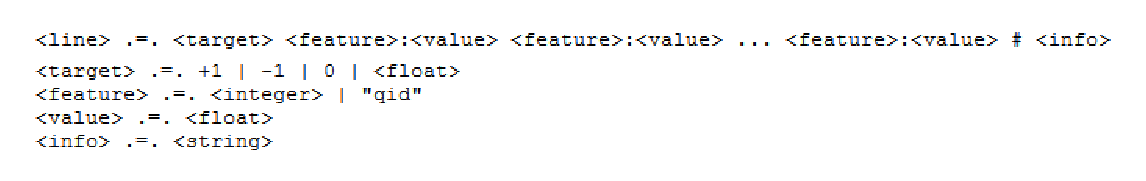
\includegraphics[width=1\textwidth]{images/svmlight}
  \caption{Svm light format.\label{fig:svmlight}}
\end{figure}

Libsvm uses internal structures such as \textit{svm\_node} and \textit{svm\_problem} to read the input file and store it internally.
After reading the input file, it calculates the Kernel matrix which is then used for finding the maximum margin classifier.

An input file consists of samples.  
Each samples consists of target and features.

Each and every feature is stored in a svm\_node with index and value.
All these are stored in an array per sample.
This structure doesn't easily translate to vector representation and hence plugging in the GPU based gram matrix calculation or SMO implementation.

\section{Proposed solution}
We propose two different approaches for implementing SVMs using GPU\@.

\begin{enumerate}
\item Implement the Sequential Minimal Optimization method for solving the dual problem using GPUs and OpenMpi.
\item Implement the Gram matrix calculation using GPU and use libsvm to solve the actual SMO problem.
\end{enumerate}

\section{Experimental Setup}
We use cuda2 and cuda5 machines for all the experiments.
The cuda machines got surprisingly slow in the last few days and I resorted to using NYU HPC machines with Titan GPU for later experiments.
We also use MNIST~\cite{lecun1998mnist} dataset for all the experiments.

MNIST dataset contains a total of 60,000 samples for test and 10,000 samples for test.
We track the time, accuracy of test after training on 600, 1200, 6000, 15000, 30000 and 60000 samples.


I started out with implementing the SMO in GPU following the reference implementation at~\cite{dpsvm}.
The reference implementation uses OpenMPI, CUDA, Thrust, and BLAS (cuBLAS, cBLAS, and BLAS) libraries.
Even though I had the reference implementation, understanding and reimplementing the reference implementation proved to be a difficult task.
After working on the reference implementation for two days, I started to search for alternate methods to speedup the SVM classifier.


Libsvm computes the kernel function and caches them using a LRU cache.
The LRU cache has a fixed maximum size.  
So, if we have a huge amount of data, then the number of rows from the kernel matrix that can be cached will be less.
Whenever an entry has to be created in the cache, a new row of the kernel has to be calculated and pushed into the cache.

\section{Experimental Result \& Analysis}

We implemented matrix multiplication for generating the gram matrix similar to the implementation given in~\cite{matrixmuleg}.
We were able to get the same accuracy for both implementations.

Since the implementation I am using was cuda blas implementation, I cound't find a way to optimize it further.  
Also, we can observe that there are huge performance improvement in case of larger datasets.

\begin{figure}[ht!]
  \centering
  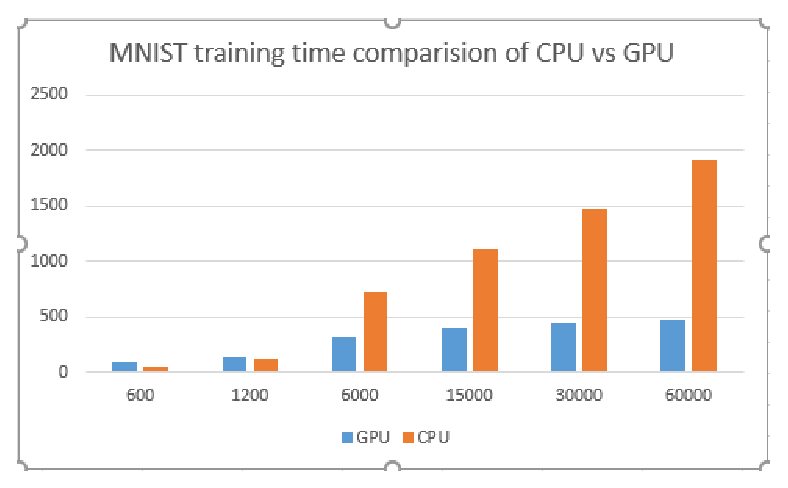
\includegraphics[width=1\textwidth]{images/gpuvscpu}
  \caption{Mnist training gpu vs cpu performance.\label{fig:gpuvscpu}}
\end{figure}

\section{Conclusions}


\bibliographystyle{plain}
\bibliography{references}

\end{document}
